\documentclass[../main-sheet.tex]{subfiles}
\usepackage{../style}
\graphicspath{ {../img/} }
\backgroundsetup{contents={}}
\everymath{\displaystyle}
\begin{document}
\chapter{Separation Axioms}
\section{\(T_0\) Space}
\begin{defn}
    A topological space \(\xt\) is said to be a \(T_0\) space iff given any two distinct points \(x,y\) in \(X\), there exists either an open set \(U\) containing \(x\) but not \(y\) or an open set \(v\) containing \(y\) but not \(x\).
\end{defn}
\begin{ex}
    Every discrete space is a \(T_0\) space. Because for any two points \(x\neq y\) in \(X\), there always exists an open \(\set{x}\) containing \(x\) but not \(y\). But indiscrete space is not \(T_0\) space because the only nonempty open set in this space is \(X\) itself.
\end{ex}
\begin{ex}
    Any co-finite topological space \(xt\) is a \(T_0\) space for 
    \begin{enumerate}[label={Case \roman*.}]
        \item \(X\) is finite. In this case \(\tau=\mathcal{P}(X)\), a discrete space, and so \(\xt\) is \(T_0\) space.
        \item \(X\) is infinite. In this case, let \(x,y\in X\) with \(x\neq y\). Then \(X-\set{x} \) is an open set containing \(y \) but not \(x\).
    \end{enumerate}
\end{ex}
\begin{ex}
    Every metric space is \(T_0\) space. For let \((X,d)\) be a metric space and \(\tau\) be a topology induced by the metric \(d\).\\ The open set
\end{ex}
\begin{figure}
\centering    
    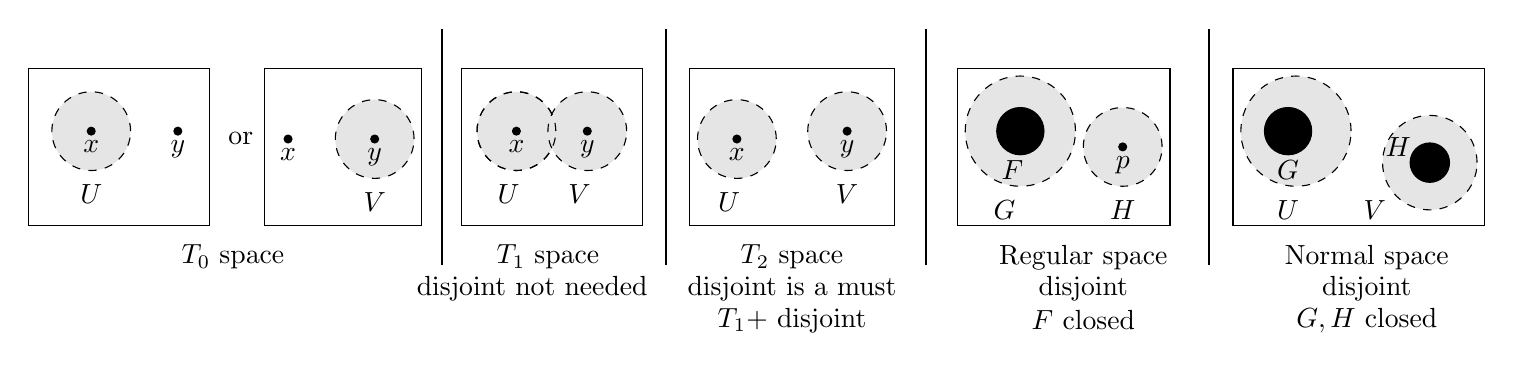
\begin{tikzpicture}
        \draw (-5,0) rectangle (-2.7,2);
        \draw[dashed,fill=gray!20] (-4.2,1.2) circle[radius=.5];
        \node at (-0.6,0.3) {$V$};
        \draw[fill=black] (-4.2,1.2) circle[radius=.05] node[below] {$x$};
        \draw[fill=black] (-3.1,1.2) circle[radius=.05] node[below] {$y$};
        \node at (-2.3,1.1) {or};
        \draw (-2,0) rectangle (0,2);
        \draw[dashed,fill=gray!20] (-0.6,1.1) circle[radius=.5];
        \node at (-4.2,0.4) {$U$};
        \draw[fill=black] (-1.7,1.1) circle[radius=.05] node[below] {$x$};
        \draw[fill=black] (-0.6,1.1) circle[radius=.05] node[below] {$y$};
        \draw[thick] (.25,-.5)--(.25,2.5);
        
        \draw (0.5,0) rectangle (2.8,2);
        \draw[dashed,fill=gray!20] (1.2,1.2) circle[radius=.5];
        \draw[dashed,fill=gray!20] (2.1,1.2) circle[radius=.5];
        \draw[dashed] (1.2,1.2) circle[radius=.5];
        \node at (1.1,0.4) {$U$};
        \node at (2,0.4) {$V$};
        \draw[fill=black] (1.2,1.2) circle[radius=.05] node[below] {$x$};
        \draw[fill=black] (2.1,1.2) circle[radius=.05] node[below] {$y$};
        \draw[thick] (3.1,-0.5)--(3.1,2.5);
        
        \draw (3.4,0) rectangle (6,2);
        \draw[dashed,fill=gray!20] (4,1.1) circle[radius=.5];
        \draw[dashed,fill=gray!20] (5.4,1.2) circle[radius=.5];
        \node at (3.9,0.3) {$U$};
        \node at (5.4,0.4) {$V$};
        \draw[fill=black] (4,1.1) circle[radius=.05] node[below] {$x$};
        \draw[fill=black] (5.4,1.2) circle[radius=.05] node[below] {$y$};
        \draw[thick] (6.4,-0.5)--(6.4,2.5);
    
        \draw (6.8,0) rectangle (9.5,2);
        \draw[dashed,fill=gray!20] (7.6,1.2) circle[radius=.7];
        \draw[dashed,fill=gray!20] (8.9,1) circle[radius=.5];
        \node at (7.4,0.2) {$G$};
        \node at (8.9,0.2) {$H$};
        \node at (7.5,0.7) {$F$};
        \draw[fill=black] (7.6,1.2) circle[radius=.3];
        \draw[fill=black] (8.9,1) circle[radius=.05] node[below] {$p$};
        \draw[thick] (10,-0.5)--(10,2.5);
        
        \draw (10.3,0) rectangle (13.5,2);
        \draw[dashed,fill=gray!20] (11.1,1.2) circle[radius=.7];
        \draw[dashed,fill=gray!20] (12.8,0.8) circle[radius=.6];
        \node at (11,0.2) {$U$};
        \node at (12.1,0.2) {$V$};
        \node at (11,0.7) {$G$};
        \node at (12.4,1) {$H$};
        \draw[fill=black] (11,1.2) circle[radius=.3];
        \draw[fill=black] (12.8,0.8) circle[radius=.25];
        
        \node at (-2.4,-0.4) {$T_0$ space};
        \node at (1.6,-0.4) {$T_1$ space};
        \node at (1.4,-0.8) {disjoint not needed};
        \node at (4.7,-0.4) {$T_2$ space};
        \node at (4.7,-0.8) {disjoint is a must};
        \node at (4.7,-1.2) {$T_1+ $ disjoint};
        
        \node at (8.4,-0.4) {Regular space};
        \node at (8.4,-0.8) {disjoint};
        \node at (8.4,-1.2) {$F $ closed };
        
        \node at (12.0,-0.4) {Normal space};
        \node at (12.0,-0.8) {disjoint};
        \node at (12,-1.2) {$G,H $ closed };
    \end{tikzpicture}
\end{figure}
\end{document}